\section{乘法竖式}

\title[第4讲\quad 乘法竖式]{第4讲\quad 乘法竖式} 
\author{}
\date{}
\begin{frame}
    \titlepage
\end{frame}

\begin{frame}
    \frametitle{课前测}
    \textit{已知有如图竖式谜: $\ding{73} =$\underline{\hbox to 10mm{}},$\triangle =$\underline{\hbox to 10mm{}}.\\
    A. 3, 2\qquad 
    B. 6, 1\qquad 
    C. 2, 1\qquad
    D. 2, 4}
    \begin{figure}[H] 
        \centering
        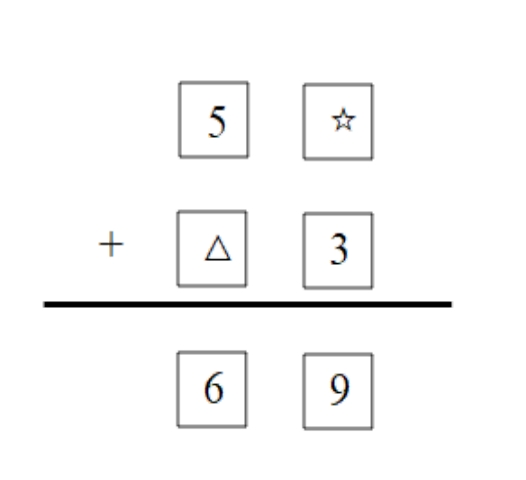
\includegraphics[width=0.4\textwidth]{./pics/Chapter_4/keqian1.png}
    \end{figure}
    % B
\end{frame}

\begin{frame}
    \frametitle{课前测}
    \textit{请问下列竖式中第二个加数是多少?\\
    A. 68\qquad 
    B. 78\qquad 
    C. 88\qquad
    D. 98}
    \begin{figure}[H] 
        \centering
        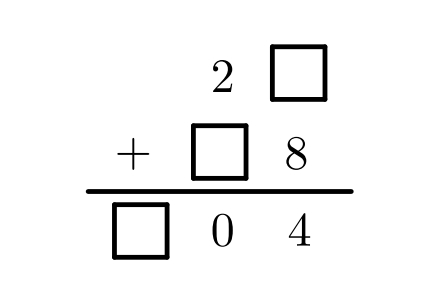
\includegraphics[width=0.4\textwidth]{./pics/Chapter_4/keqian2.png}
    \end{figure}
    % B
\end{frame}

\begin{frame}
    \frametitle{课前测}
    \parbox{0.9\textwidth}{在下图的加法算式中,每个字母代表一个数字,不同的字母代表不同的数字,那么EFFC代表的四位数是\underline{\hbox to 10mm{}}.\\
    A. 1006\qquad 
    B. 1007\qquad 
    C. 1008\qquad
    D. 1009}
    \begin{figure}[H] 
        \centering
        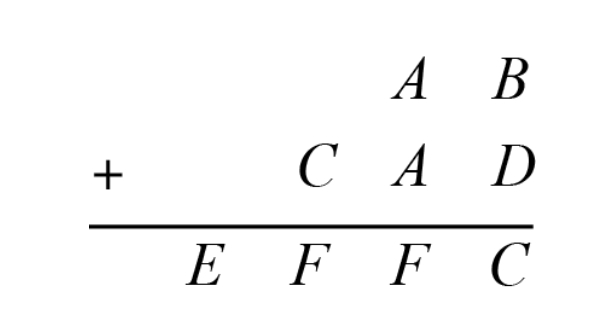
\includegraphics[width=0.4\textwidth]{./pics/Chapter_4/keqian3.png}
    \end{figure}
    % D
\end{frame}

\begin{frame}
    \frametitle{知识梳理}
\end{frame}

\begin{frame}
    \frametitle{MISSION 1}
    \textit{在列乘法竖式的时候,有哪些地方需要注意?\\}
    \textit{1. 数位对齐\\
        2. 个位算起\\
        3. 满十进一}
\end{frame}

\begin{frame}
    \frametitle{探索1}
    \textit{(1) $56\times 9 = $\\
        (2) $314\times 2 = $\\
        (3) $732\times 4 = $\\
        (4) $284\times 6 = $\\
        (5) $1234\times 7 = $\\}
\end{frame}

\begin{frame}
    \frametitle{探索2}
    \textit{(1) $506\times 3 = $\\
        (2) $4003\times 7 = $\\
        (3) $5036\times 8 = $\\
        (4) $4320\times 8 = $}
\end{frame}

\begin{frame}
    \frametitle{探索3}
    \textit{(1) $55\times 29 = $\\
        (2) $18\times 63 = $\\
        (3) $123\times 45 = $\\
        (4) $721\times 28 = $}
\end{frame}

\begin{frame}
    \frametitle{捉虫时刻}
    \textit{请你给企鹅治病,并开出处方.}
    \begin{figure}[H] 
        \centering
        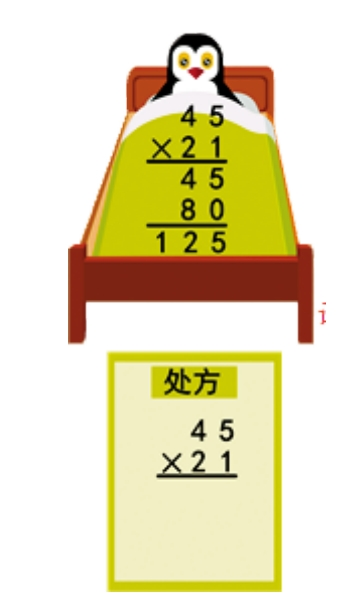
\includegraphics[width=0.3\textwidth]{./pics/Chapter_4/zhuochong.png}
    \end{figure}
\end{frame}

\begin{frame}
    \frametitle{探索4}
    \textit{(1) $150\times 270 = $\\
        (2) $3600\times 250 = $\\
        (3) $2030\times 140 = $\\
        (4) $102\times 3040 = $}
\end{frame}

\begin{frame}
    \frametitle{探索5}
    \textit{(1) $38\times 32 + 37\times 33 + 36\times 34$}
\end{frame}

\begin{frame}
    \frametitle{探索5}
    \textit{(2) $12\times 92 + 22\times 82 + 32\times 72$}
\end{frame}

\begin{frame}
    \frametitle{MISSION 2}
    \textit{同学们,你能说说加、减、乘、除这四则运算的优先级么 ?}
\end{frame}

\begin{frame}
    \frametitle{探索6}
    \textit{双面龟的壳上有一副神秘地图,巨整指出这是标记了三片龙鳞位置的山海图.图中显示金鳞距离出发点130米,火鳞距离出发点320米,水鳞距离出发点250米,小鲤鱼和它的小伙伴们一共6人,2人一组出发寻找宝藏,请问各组到达目的地时全组人一共走的路程是多少米?}
    % 1200
\end{frame}

\begin{frame}
    \frametitle{探索7}
    \textit{艾迪去文具店帮老师买文具,文具的单价如下:自动铅笔4元一支,文具盒26元一个,钢笔45元一支,书包128元一个,艾迪要买32支铅笔,24个文具盒,65支钢笔,9个书包,请问艾迪要花多少钱 ?}
    % 4829
\end{frame}

\begin{frame}
    \frametitle{探索8}
    \textit{鲤鱼湖中突然出现了一个奇怪的植物一刺刺球,由于没有天敌,刺刺球开始大量扩散.于是全村的居民出动,分为4组开始清理刺刺球.已知第1组有47人,每人每天可以清理21个刺刺球,第2组有94人,每人每天可以清理18个刺刺球,第3组有57人,每人每天可以清理53个刺刺球,第4组不仅没有清理好刺刺球,反而由于操作失误,使得刺刺球每天增加100个,请问全村一天一共可以使刺刺球减少多少个?}
    % 5600
\end{frame}